% =====================================================================
%  talk.tex  --  MARBLE 2026 conference talk.
%
%  "Optimal Block Time for AMM Liquidity Providers under Jump-Diffusion
%  Prices", 7th International Conference on Mathematical Research for
%  Blockchain Economy, Limassol, 16-18 September 2026.
%
%  Slot: 15-17 minutes of talk plus 3-5 minutes of Q&A. The main deck is
%  17 content slides, roughly a minute each; everything cut to fit lives
%  after \appendix as backup slides for the discussion.
%
%  Build:  make        (or: pdflatex talk && pdflatex talk)
% =====================================================================
\documentclass[10pt,xcolor=x11names,aspectratio=169]{beamer}
\usepackage{zhaw-theme}
% =====================================================================
%  presentation-info.tex  --  shared metadata for the MARBLE 2026 talk.
% =====================================================================
\newcommand{\zhawcoursetitle}{Optimal Block Time under Jump-Diffusion}
\renewcommand{\zhawinstitute}{ZHAW School of Engineering}
\renewcommand{\zhawunit}{}                     % <- fill in the institute if you want it in the footer
\newcommand{\zhawdocname}{\zhawcoursetitle}

\renewcommand{\zhawpresenter}{Nils Bundi}

% Details for the closing slide (\closingslide).
% Placeholders -- check before printing the closing slide.
\renewcommand{\zhawposition}{Researcher}
\renewcommand{\zhawaddress}{Technikumstrasse 9 \textbar\ PO Box\\8401 Winterthur, Switzerland}
\renewcommand{\zhawphone}{+41 58 934 71 71}   % ZHAW switchboard; replace with your direct line
\renewcommand{\zhawemail}{bund@zhaw.ch}
\renewcommand{\zhawweb}{www.zhaw.ch/engineering}

% Standard title-page block.
\author{\zhawpresenter}
\institute{\zhawinstitute}
\date{MARBLE 2026 \textbar\ Cyprus \textbar\ 16--18 September 2026}

% Footer (left cell). The organisational unit is left out of the corporate-design
% line here, since this is a conference talk rather than an internal deck.
\lfooter{\zhawinstitute\ \textbar\ \zhawdocname}


\usepackage{mathtools}

\newcommand{\dt}{\Delta t}
\newcommand{\E}{\mathbb{E}}
\newcommand{\Prob}{\mathbb{P}}
\newcommand{\R}{\mathbb{R}}
\newcommand{\bound}{\mathrm{bound}}
\newcommand{\1}{\mathbf{1}}
\newcommand{\bpyr}{\,\text{bp/yr}}

% The theme's closing slide prints a phone number; this one does not.
\makeatletter
\renewcommand{\closingslide}{%
  {\zhaw@nightcanvas
   \begin{frame}
     \usebeamerfont{orginfo}%
     \zhawuniversity\par\vskip 2.5mm
     \textbf{\zhawinstitute}\par\vskip 2.5mm
     \zhawpresenter\\\zhawposition\\\zhawaddress\\
     \zhawemail\\\zhawweb\par
     \vfill
   \end{frame}}}
\makeatother

% The theme splits the footer .58/.27/.15, which puts the middle cell at 0.715
% of the page. Equal outer cells centre it instead.
\makeatletter
\setbeamertemplate{footline}{%
  \leavevmode
  \begin{beamercolorbox}[wd=.425\paperwidth,ht=2.25ex,dp=\@footermargin,left,leftskip=\@lrmargin]{lfooter}%
    \usebeamerfont{footline}\@lfooter
  \end{beamercolorbox}%
  \begin{beamercolorbox}[wd=.15\paperwidth,ht=2.25ex,dp=\@footermargin,center]{mfooter}%
    \usebeamerfont{footline}\@mfooter
  \end{beamercolorbox}%
  \begin{beamercolorbox}[wd=.425\paperwidth,ht=2.25ex,dp=\@footermargin,right,rightskip=\@lrmargin]{rfooter}%
    \usebeamerfont{footline}\insertframenumber
  \end{beamercolorbox}%
}
\makeatother

\mfooter{MARBLE 2026}
\title{Optimal Block Time for\\ AMM Liquidity Providers\\ under Jump-Diffusion Prices}
\subtitle{MARBLE 2026 --- 7th International Conference on\\ Mathematical Research for Blockchain Economy}

\begin{document}

% ---------------------------------------------------------------- title
\begin{frame}[plain,noframenumbering]\titlepage\end{frame}

% =====================================================================
\section{The case for faster blocks}
% =====================================================================

\begin{frame}{Two live conversations about how fast a chain should be}
  \begin{rwexample}[Arbitrum Research --- ``The power of faster blocks'' (Felten, May 2024)]
    ``Arbitrum's $250$ millisecond block time leads to $65\%$ lower
    arbitrage loss compared to a $2$ second block time.''
    \blockmarker{\weblink{https://research.arbitrum.io/t/the-power-of-faster-blocks/9609}%
      {research.arbitrum.io/t/the-power-of-faster-blocks/9609}}
  \end{rwexample}
  \begin{rwexample}[EIP-7782 ``Reduce Block Latency'' --- $12$ s $\to$ $6$ s, drafted for Glamsterdam]
    ``More frequent blocks decrease LVR (Loss Versus Rebalancing), which
    improves the economics for liquidity providers. More liquidity means lower
    spreads.''
    \blockmarker{\weblink{https://eips.ethereum.org/EIPS/eip-7782}%
      {eips.ethereum.org/EIPS/eip-7782}}
  \end{rwexample}
  Both rest on the same result. Both, on the numbers below, overstate the gain
  --- by roughly a factor of two.
\end{frame}

\begin{frame}{What an automated market maker is}
  \begin{columns}[T]
    \begin{column}{0.53\textwidth}
      A smart contract, or pool, holds reserves $x$ of $X$ and $y$ of $Y$. Anyone may swap against
      it. There is no order book and nobody quoting.
      \begin{itemize}
        \item The rule is an invariant, $x_ty_t = L$: a swap is any move
              along that curve, and the curve alone decides what you get.
        \item The pool's price is the curve's slope, $P = y/x$. Nothing else
              sets it --- the pool cannot see the outside market.
        \item LPs supply the reserves and earn a swap fee; they never quote or
              cancel.
      \end{itemize}
    \end{column}
    \begin{column}{0.45\textwidth}
      \centering
      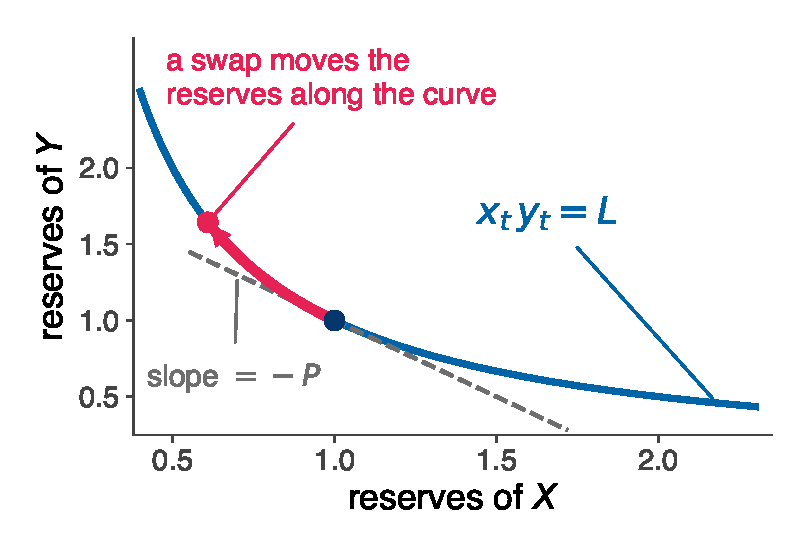
\includegraphics[width=\linewidth]{fig_cpmm}
    \end{column}
  \end{columns}
  \begin{pitfall}[Where the loss comes from]
    An external move leaves the pool's marginal price stale. Arbitrage restores its
    price, but the trade executes along the convex curve below the
    new price. The LP bears the difference.
  \end{pitfall}
\end{frame}

\begin{frame}{What we know about LVR}
  Milionis et al.\ (2022, 2023) named that loss loss-versus-rebalancing
  (LVR), and shaped how its relationship with block time is understood today.
  \begin{itemize}
    \item Under geometric Brownian motion, a constant-product pool loses at the
          rate $\sigma^2 V/8$, independent of the block time.
    \item Add a swap fee $\gamma$ and Poisson blocks of mean $\dt$
          (Milionis et al., 2023): the rate is multiplied by
          $F(\kappa)$, $\kappa = \gamma/(\sigma\sqrt{\dt})$ ---
          the stationary probability that an arriving block offers a
          \emph{profitable} trade.
    \item $F(\kappa) \sim \sigma\sqrt{\dt}/(\sqrt2\gamma) \to 0$ as $\dt\to0$.
          That $\sqrt{\dt}$ is where Arbitrum's $65\%$ comes from, and the
          ${\sim}29\%$ implied by halving Ethereum's slot.
  \end{itemize}
  \begin{pitfall}[The primitive all of this assumes]
    Milionis et al. assume a \emph{continuous} reference price, and
    crypto prices are not (Scaillet et al., 2020, Saef et al., 2024). 
    A jump of size $J$ opens a gap of size $J$ whatever the block time.
  \end{pitfall}
\end{frame}

\begin{frame}{Contributions}
  \begin{enumerate}
    \item \hl{Two LVR channels.} Once the price can jump, the loss
          separates into a channel the block schedule governs and one it cannot
          reach (Theorems~1--2).
    \item \hl{A jump induced floor.} Faster blocks clear a jump gap
          sooner, never smaller. So the loss rate stops falling at a strictly
          positive level (Theorem~3).
    \item \hl{A planner's objective.} Blocks cost something to
          produce. A planner's welfare problem puts the cost in relation with the LVR loss (Theorem~4).
    \item \hl{Empirical calibration.} Magnitudes of loss, cost and optimum are computed from six 
          years of ETH/USDT tick data, and Ethereum's issuance.
  \end{enumerate}
  \begin{takeaway}[Headline]
    At Ethereum's $12$~s, LPs lose $471\bpyr$, $125$ of it beyond any
    schedule's reach; the optimum sits near $8$~s. So the two proposals I opened
    with are worth \hl{$35\%$} and \hl{$14\%$}, not $65\%$ and $29\%$.
  \end{takeaway}
\end{frame}

% =====================================================================
\section{Two channels, and a floor}
% =====================================================================

\begin{frame}{Setup}
  Milionis et al.\ with one primitive changed: the reference price jumps.
  \[
    \frac{dS_t}{S_{t-}} \;=\; \mu\,dt + \sigma\,dW_t + (e^{J_t}-1)\,dN_t,
    \qquad N \text{ Poisson}(\lambda),\quad J \sim \nu .
  \]
  \begin{itemize}
    \item CPMM, $x_ty_t = L$, price $P = y/x$, pool value $V(P) = 2\sqrt{LP}$.
    \item Fee $\gamma$ in log-price units $\Rightarrow$ no-arbitrage band
          $\{|\log S - \log P| \le \gamma\}$.
    \item Blocks arrive Poisson at rate $1/\dt$, so $\dt$ is the \emph{mean}
          time between them.
    \item $\mathrm{LVR}(T) = \int_0^T V'(P_{s-})\,dP_s - [V(P_T)-V(P_0)]$;
          rate $\ell = \E_t[d\mathrm{LVR}_t]/dt$.
    \item $\nu$ finite activity with $\int (e^{j/2}-1)^2 \nu(dj) < \infty$;
          Merton $J\sim\mathcal N(m,\delta^2)$ the running instance.
  \end{itemize}
  \begin{block}{What is general and what is not}
    Theorems 1, 2, 4 hold for arbitrary $\nu$; Proposition~1 and Theorem~3 need symmetry; 
    Gaussianity is not assumed anywhere.
  \end{block}
\end{frame}

\begin{frame}{Theorem 1 --- the zero-fee decomposition}
  In the continuous-arbitrage limit ($\gamma=0$, $\dt\to0$), $P_t \equiv S_t$
  and LVR is the It\^o--L\'evy remainder of $V(S_t)$:
  \begin{block}{}
    \[
      \ell \;=\;
        \underbrace{\frac{\sigma^2}{8}V(S_t)}_{\text{diffusion-LVR}}
        \;+\;
        \underbrace{\frac{\lambda}{2}V(S_t)\,\E\big[(e^{J/2}-1)^2\big]}_{\text{jump-LVR}}
    \]
  \end{block}
  For Merton, $\E[(e^{J/2}-1)^2] = e^{m+\delta^2/2} - 2e^{m/2+\delta^2/8} + 1
  \ge 0$, zero iff $J \equiv 0$.
  \vspace{-1mm}

  \begin{columns}[T]
    \begin{column}{0.48\textwidth}
      \begin{block}{What to watch}
        This is the $\dt\to0$ limit, so \emph{neither} term shows a $\dt$ yet.
        What matters is where each comes from: the first from the variance of a
        continuous path, the second from the jump law alone. Put blocks back in
        and only the first picks up a discount.
      \end{block}
    \end{column}
    \begin{column}{0.48\textwidth}
      \begin{block}{Measure}
        The drift cancels between the two terms, so no normalisation of $\mu$
        is needed --- but with jumps the rate is \emph{not} measure-independent.
        This is a physical-measure statement, calibrated against realised
        prices.
      \end{block}
    \end{column}
  \end{columns}
\end{frame}

\begin{frame}{The mispricing process}
  \begin{columns}[T]
    \begin{column}{0.38\textwidth}
      A fee opens a gap between reference and pool:
      \[ z_t \;:=\; \log(S_t/P_t). \]
      \begin{itemize}
        \item \textbf{No-arbitrage band} $|z|\le\gamma$: inside it, no trade
              covers the fee.
        \item At a block, trade iff $|z|>\gamma$ --- and only out to the
              \emph{near band edge}, not to $0$.
      \end{itemize}
    \end{column}
    \begin{column}{0.60\textwidth}
      \centering
      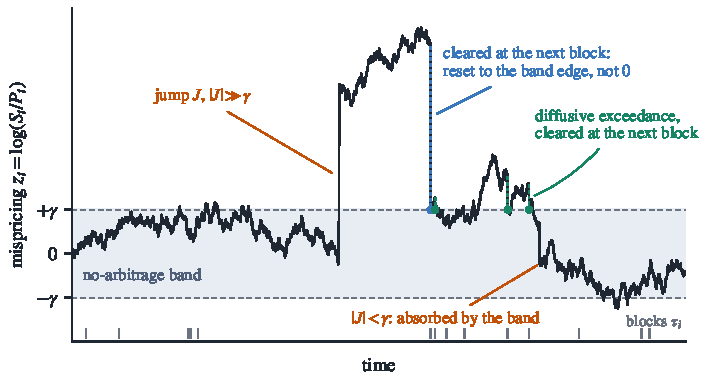
\includegraphics[width=\linewidth]{fig_mispricing_path}
    \end{column}
  \end{columns}
\end{frame}

\begin{frame}{The two channels, separately}
  \begin{columns}[T]
    \begin{column}{0.49\textwidth}
      \textbf{Diffusion (Lemma 1).} At $\lambda=0$ the stationary law is
      uniform on the band with exponential tails, so
      \[
        \ell_{\mathrm{diff}} = \tfrac{\sigma^2}{8}V\cdot F(\kappa),
        \quad F(\kappa) = \frac{1}{1+\sqrt2\,\kappa}
      \]
      with $\kappa = \gamma/(\sigma\sqrt{\dt})$; $F(\kappa) =
      \Prob_\pi(|z|>\gamma)$, strictly decreasing, $F(\kappa)\to0$.
    \end{column}
    \begin{column}{0.49\textwidth}
      \textbf{Jumps (Lemma 2).} Each jump is charged once, on its excess
      over the band, at rate $\lambda$:
      \[
        \begin{gathered}
          \ell_{\mathrm{jump}} = \lambda V\cdot G_\nu(\gamma),\\[2pt]
          G_\nu(\gamma) = \tfrac18\E_\nu\big[(|J|-\gamma)^2\1\{|J|>\gamma\}\big]
        \end{gathered}
      \]
      a functional of $\nu$ alone. For symmetric Merton,
      $G = \tfrac{\delta^2}{8}\Psi(\gamma/\delta)$.
    \end{column}
  \end{columns}
  \medskip
  \begin{block}{The fee discount is different on each channel}
    Both channels are trimmed by the fee --- but by $F(\gamma/\sigma\sqrt{\dt})$
    on one and by $\Psi(\gamma/\delta)$ on the other. Only the first
    contains $\dt$, because the size of a jump is set by $\delta$, not by how
    long the block lasted.
  \end{block}
\end{frame}

\begin{frame}{Theorem 2 --- the separated rate}

  I define the separated rate $\ell_0$ and write the LVR rate as the sum of 
  the separated rate and an error term $\mathcal{E}(\dt)$.

  \begin{block}{}
    \[
      \ell(\dt) \;=\; \ell_0(\dt) + \mathcal{E}(\dt),
      \qquad
      \ell_0(\dt) := \frac{\sigma^2}{8}V\cdot F\!\Big(\frac{\gamma}{\sigma\sqrt{\dt}}\Big)
      \;+\; \lambda V \cdot G_\nu(\gamma).
    \]
  \end{block}
  \medskip

  The error $\mathcal{E}(\dt)$ captures a number of effects that are not in the separated rate.
  This term needs to be bounded to make the decomposition useful, which is what Proposition~1 does.
  \medskip

  \textbf{Proposition 1} Under a mixing condition, the error term $\mathcal{E}(\dt)$ is bounded by
  closed-form expressions from below and above; 
  \begin{itemize}
    \item The mixing condition is numerically verified for symmetric jump laws and relevant regimes.
    \item The bounds derive from six terms: interaction, block clock, single-jump thinning,
          multi-jump, curvature residual, stationary law.
    \item The bracket is tight --- under $0.29\%$ of the rate
          across the empirically relevant regime.
  \end{itemize}
\end{frame}

\begin{frame}{Theorem 3 --- an exact floor}
  Let $\nu$ be symmetric and satisfy $\E[g(\sum_1^k J)] \ge k\,\E[g(J)]$ for
  every $k$ (Merton with $m=0$ does). Then for \emph{every} $\dt>0$
  \medskip
  
  \begin{block}{}
    \[
      \ell(\dt)\;\ge\;\lambda V\,G_\nu(\gamma)\;=\;\inf_{\dt'>0}\ell_0(\dt')\;>\;0
    \]
  \end{block}
  \medskip

  \textbf{Corollary 1.} $\ell_0$ is strictly increasing and the floor is
          approached only as $\sqrt{\dt}$: halving the block time removes at
          most $29\%$ of the diffusion term.
  \medskip

  \begin{takeaway}[Key takeaway]
    The jump channel establishes a strictly positive floor to the LVR rate, beyond 
    which block-time reductions do not help. Approaching the floor is slow, at the 
    rate $\sqrt{\dt}$.
  \end{takeaway}
\end{frame}

% =====================================================================
\section{The planner's optimum, and the numbers}
% =====================================================================

\begin{frame}{The planner's welfare problem}
  Shorter blocks are always better, down to the floor --- so why not $\dt\to0$? Because
  blocks are not free.
  \begin{itemize}
    \item Each block costs fixed work whatever it carries --- gossip, signature
          aggregation, the commit round --- so the chain-level rate is
          $R(\dt) = r/\dt$.
    \item That cost is not observable, so I proxy $r$ by issuance: 
          it overstates where it subsidises growth and understates where fees 
          and MEV pay validators.
    \item A pool of TVL $V$ inherits a share by value secured:
          $c/\dt$ with $c := r\,V/V_{\text{chain}}$.
  \end{itemize}
  \begin{block}{}
    \[
      \min_{\dt>0}\; W(\dt) \;=\; \underbrace{\ell_0(\dt)}_{\text{LVR}}
      \;+\; \underbrace{c/\dt}_{\text{cost of consensus}}
    \]
  \end{block}
  \begin{takeaway}[The trade-off]
    Two terms, two forces: the LVR pulls to the floor,
    the other grows without bound.
  \end{takeaway}
\end{frame}

\begin{frame}{Theorem 4 --- netting LVR against what a block costs}
  Minimising $W$ gives a first-order condition in $\eta = \sqrt2\,\kappa$:
  \begin{block}{}
    \[
      \eta^{\mathrm{opt}}\big(1+\eta^{\mathrm{opt}}\big)^2 = \frac{V\gamma^2}{8c},
      \qquad
      \dt^{\mathrm{opt}} = \frac{2\gamma^2}{\sigma^2(\eta^{\mathrm{opt}})^2},
    \]
  \end{block}
  a cubic with a unique positive root, closed form by Cardano.
  \medskip

  \textbf{Importantly}, the optimum is a property of the block time
and the fee tier only;
  \begin{itemize}
    \item $\partial\dt^{\mathrm{opt}}/\partial\lambda =
          \partial\dt^{\mathrm{opt}}/\partial m =
          \partial\dt^{\mathrm{opt}}/\partial\delta = 0$: the jump
          parameters do not enter the first-order condition.
    \item $\partial\dt^{\mathrm{opt}}/\partial V = 0$: the pool size does not enter either.
  \end{itemize}
  \begin{pitfall}[What the remainder does to it]
    That invariance is a property of $\ell_0$; $\mathcal E$ carries both
    $\lambda$ and $\dt$. Bounding it directly puts any exact minimiser in
    $[7.3,\,9.9]$~s --- the range over which $W$ is within $1\bpyr$ of its
    minimum anyway.
  \end{pitfall}
\end{frame}

\begin{frame}{Calibration}
  % NB: do not open this body with a brace group -- beamer would read it as the
  % frame subtitle, which this theme does not typeset, and the text disappears.
  \textbf{Price.} Binance ETH/USDT $5$-minute closes, Jan 2020 -- Jun 2026
  ($2{,}373$ days, $682{,}946$ bars):
  \begin{itemize}
    \item $\sigma = 0.8156$, the continuous part of realised variance.
    \item $\lambda = 283.3$/yr and $\delta = 0.0192$, from Lee--Mykland jump
          detection.
    \item $m = 0$: the sample gives $\hat m = -0.0012$, with a $99\%$ interval
          that contains zero.
  \end{itemize}
  \medskip

  \textbf{Consensus cost.} Ethereum's own issuance, as a proxy for the resource
  cost of producing a block:
  \begin{itemize}
    \item Gross issuance ${\sim}\$1.7$B/yr against $V_{\text{chain}} \approx
          \$208$B, scaled by $0.83$ because staked supply (${\sim}30\%$) sits
          above Drake's security-optimal quarter.
    \item Attributed to the pool pro-rata by value secured,
          $V/V_{\text{chain}} = 4.8\times10^{-6}$, giving
          $c \approx \$260\times10^{-5}$ per block.
  \end{itemize}
  \medskip
  
  \textbf{Modelling choices.} $\gamma = 5$~bp (Uniswap $0.05\%$ tier),
  $V = \$1$M.
\end{frame}

\begin{frame}{The rate across deployed block times --- and the optimum}
  \begin{columns}[T]
    \begin{column}{0.50\textwidth}
      \small
      \begin{tabular}{lrrr}
        \toprule
        Chain & $\dt$ & $\ell$ (bp/yr) & diff.\ share \\
        \midrule
        Ethereum L1 & $12$ s   & $471$ & $73\%$ \\
        Base / OP L2 & $2$ s   & $312$ & $60\%$ \\
        Solana      & $400$ ms & $221$ & $43\%$ \\
        Arbitrum    & $250$ ms & $203$ & $38\%$ \\
        App-chain   & $50$ ms  & $162$ & $23\%$ \\
        \midrule
        Jump floor  & ---      & $125$ & $0\%$ \\
        \bottomrule
      \end{tabular}
    \end{column}
    \begin{column}{0.47\textwidth}
      \begin{itemize}
        \item Ceiling $\sigma^2V/8 = 832\bpyr$; floor $\lambda VG = 125$.
        \item A $240\times$ cut, $12$~s $\to$ $50$~ms, removes only $89\%$ of
              the diffusion term and leaves the rate $29\%$ above the floor.
        \item The channels are equal at $\dt_\times \approx 0.75$~s.
      \end{itemize}
    \end{column}
  \end{columns}
  \medskip

  \begin{takeaway}[Where the optimum lands]
    Theorem~4 gives $\dt^{\mathrm{opt}} \approx 8.4$~s --- two-thirds of Ethereum's slot,
    and far above sub-second timing. The gain is small and the optimum shallow:
    $W$ falls $539 \to 533\bpyr$, under $2\%$, and stays within $1\bpyr$ of its
    minimum over $[7.4,\,9.7]$~s.
  \end{takeaway}
\end{frame}

% =====================================================================
\section{What this means, and what it does not}
% =====================================================================

\begin{frame}{Policy}
  \begin{itemize}
    \item Price jumps set a floor beyond which block time reductions do not increase LP welfare.
    \item The diffusion channel stays material into the low-millisecond range ---
          so the block time optimum is bound by the cost of a block, not by the jump channel.
    \item The block time optimum is invariant in pool size and jump regime.
    \item Once the floor does bind, the remaining LP-side levers are not the
          schedule:
      \begin{itemize}
        \item fee-tier design --- higher $\gamma$ reduces both channels, but also reduces
              trade volume, price accuracy and fee revenue (both LP and protocol);
        \item batch auctions --- clear a batch at one uniform price; no
              stale quote left standing to race against;
        \item auction-managed AMMs --- keep the quote, but sell the right
              to arb it; the rent goes to LPs.
      \end{itemize}
  \end{itemize}
  \begin{rwexample}[Back to the two proposals]
    Arbitrum, $2$~s $\to$ $250$~ms: the model gives $312 \to 203\bpyr$, a $35\%$ cut (not $65\%$).\\
    EIP-7782, $12$~s $\to$ $6$~s: the model gives $471 \to 403\bpyr$, a
    $14\%$ cut (not $29\%$).\\
    Both fail to price the jump channel.
  \end{rwexample}
\end{frame}

\begin{frame}{Conclusion}
  \begin{columns}[T]
    \begin{column}{0.49\textwidth}
      \textbf{What the model says}
      \begin{itemize}
        \item $125\bpyr$ --- the jump floor. Exact for symmetric $\nu$, at
              every block time.
        \item $471\bpyr$ at Ethereum's $12$~s, $73\%$ of it in the channel
              the schedule governs --- which yields only as $\sqrt{\dt}$.
        \item $8.4$~s --- the LP-side optimum, invariant in pool size and
              in the jump parameters.
      \end{itemize}
    \end{column}
    \begin{column}{0.49\textwidth}
      \textbf{What it's limitations are}
      \begin{itemize}
        \item The objective is LP-LVR only: Other factors like finality, UX, censorship resistance, MEV are not captured.
        \item Issuance is a proxy for block production cost.
        \item The arbitrageur is idealised; blocks are Poisson; the pool is full-range.
      \end{itemize}
    \end{column}
  \end{columns}
  \begin{takeaway}
    The LVR rate splits into a channel the schedule governs and one it cannot touch.
    The jump floor is genuine but distant: what binds the block time optimum is the cost 
    of a block, and the lever against it is $\gamma$.
  \end{takeaway}
\end{frame}

\questionsslide

\closingslide

% =====================================================================
%  BACKUP -- cut from the 15-17 minute deck, kept for the discussion.
% =====================================================================
\appendix

\section{Backup}

\figureslide[The optimum is shallow: $539 \to 533\bpyr$. Across plausible $c$ it
runs $0.2$--$15$~s; the jump parameters move it not at all.]%
{The objective, and its shallow optimum}{fig_welfare}

\begin{frame}{The stationary law of the mispricing}
  \centering
  \includegraphics[width=\textwidth,height=0.64\textheight,keepaspectratio]%
    {fig_stationary_law}%
  \par\vskip 1.5mm{\usebeamerfont{footline}%
    Pre-block mispricing at $\eta=2$, $\delta=5\gamma$, $\lambda\dt=0.08$.
    Without jumps $\pi_0$ is uniform on the band with exponential tails; jumps
    add a far field at the jump scale $\delta\gg\gamma$ --- the shoulder leaving
    the tail on the log scale, mass no block schedule can pull in.}
\end{frame}

\end{document}
